\section{Υπολογισμός παραγώγων με τη διακριτή συζυγή μέθοδο}

Οι παράγωγοι ευαισθησίας της $F$ ορίζονται σε διακριτή μορφή απο την εξίσωση \ref{eq:initDsens}. Σε αυτή την περίπτωση, $\vec{R}$ είναι το διάνυσμα των κομβικών υπολοίπων, που ορίζεται παρακάτω στην σχέση \ref{eq:resid}, $\vec{U}$ είναι το διάνυσμα των κομβικών τιμών του πάχους του οριακού στρώματος, και $\vec{b}$ το διάνυσμα των μεταβλητών σχεδιασμού. 


\begin{equation}
    \dfrac{\delta F}{\delta \vec{b}} = \dfrac{\partial F}{\partial \vec{b}} (=0) + \dfrac{\partial F}{\partial \vec{U}}\dfrac{\delta \vec{U}}{\delta \vec{b}}
\label{eq:initDsens}
\end{equation}

Και ως υπόλοιπο ορίζουμε την παρακάτω ποσότητα. 


\begin{equation}
 R_i = \Big(\dfrac{2}{\pi} - \dfrac{1}{2} \Big)\dfrac{U}{v}\delta_i\dfrac{d\delta}{dx}\Big |_{x=x_i} + \dfrac{\nu_0(x_i)}{v}\delta_i - \dfrac{\pi}{2}
\label{eq:resid}
\end{equation}

Έτσι, ορίζουμε τις παραγώγους των κομβικών υπολοίπων ως προς τις μεταβλητές σχεδιασμού ως:


\begin{equation}
    \dfrac{\delta \vec{R}}{\delta \vec{b}} = \dfrac{\partial \vec{R}}{\partial \vec{b}} + \dfrac{\partial \vec{R}}{\partial \vec{U}}\dfrac{\delta \vec{U}}{\delta \vec{b}} = 0
\label{eq:residDers}
\end{equation}

Πολλαπλασιάζοντας το διάνυσμα των παραγώγων των υπολοίπων με ένα διάνυσμα $\vec{\Psi}^T$ και αφαιρώντας το απο την εξίσωση \ref{eq:initDsens} προκύπτει η επαυξημένη μορφή της εξίσωσης \ref{eq:initDsens}:

\begin{equation}
\delta F_{aug} = \Big(\dfrac{\ F}{\partial \vec{U}}- \vec{\Psi}^T\dfrac{\partial \vec{R}}{\partial \vec{U}}\Big)\delta \vec{U} + \Big(\dfrac{\partial F}{\partial\vec{b}} - \vec{\Psi}^T\dfrac{\partial\vec{R}}{\partial\vec{b}}\Big)\delta\vec{b}
\label{eq:daAug}
\end{equation}

Έτσι, μπορούμε να ορίσουμε το σύστημα των εξισώσεων \ref{eq:discreteA} και με το διάνυσμα του $\vec{\Psi}^T$ που προκύπτει απο την επίλυση της \ref{eq:discreteA}, οι παράγωγοι ευαισθησίας δίνονται απο την \ref{eq:DAsens}.

\begin{equation}
\dfrac{\ F}{\partial \vec{U}}- \vec{\Psi}^T\dfrac{\partial \vec{R}}{\partial \vec{U}} = 0
\label{eq:discreteA}
\end{equation}

\begin{equation}
\delta F = \Big(\dfrac{\partial F}{\partial\vec{b}} - \vec{\Psi}^T\dfrac{\partial\vec{R}}{\partial\vec{b}}\Big)\delta\vec{b}
\label{eq:DAsens}
\end{equation}

Για την επίλυση του \ref{eq:discreteA} απαιτείται πρώτα ο υπολογισμός των παρακάτω ποσοτήτων:

\begin{itemize}
    \item $\dfrac{\partial \vec{R}}{\partial \vec{b}}\text{, διαστάσεων } \kappa \times N$
    \item $\dfrac{\partial \vec{R}}{\partial \vec{U}}\text{, διαστάσεων } \kappa \times \kappa$
    \item $\dfrac{\partial F}{\partial \vec{U}}\text{, διαστάσεων }  1 \times \kappa$
\end{itemize}

όπου, κ το πλήθος των κόμβων, και Ν το πλήθος των μεταβλητών σχεδιασμού.
\subsection{Υπολογισμός παραγώγων αντικειμενικής συνάρτησης}

Ο υπολογισμός της ποσότητας $\dfrac{\partial F}{\partial \vec{U}}$ προκύπτει εύκολα απο διαφόριση της έκφρασης της αντικειμενικής συνάρτησης \ref{eq:finalFric} ή συγκεκριμένα απο την έκφρασή της με τη μέθοδο των τραπεζίων \ref{eq:trapzFric}.

Για τον πρώτο και τον τελευταίο κόμβο, η έκφραση της παραγώγου είναι:
\begin{equation}
\begin{aligned}    
    \dfrac{\partial F}{\partial U_0} =& \dfrac{(x_1-x_0)}{2}\dfrac{\partial}{\partial U_0}\Bigg(\dfrac{U\pi\mu}{2U_0}+\dfrac{U\pi\mu}{2U_1}\Bigg)\\
    \dfrac{\partial F}{\partial U_0} =& -\dfrac{U\pi\mu}{4}\dfrac{(x_1-x_0)}{U_0^2}
\end{aligned}   
    \label{eq:pFU0}
\end{equation}

\begin{equation}
\begin{aligned}    
    \dfrac{\partial F}{\partial U_{\kappa}} =& \dfrac{(x_{\kappa}-x_{\kappa-1})}{2}\dfrac{\partial}{\partial U_{\kappa}}\Bigg(\dfrac{U\pi\mu}{2U_{\kappa}}+\dfrac{U\pi\mu}{2U_{\kappa-1}}\Bigg)\\
    \dfrac{\partial F}{\partial U_{\kappa}} =& -\dfrac{U\pi\mu}{4}\dfrac{(x_{\kappa}-x_{\kappa-1})}{U_{\kappa}^2}
\end{aligned}   
    \label{eq:pFUk}
\end{equation}


Και για τους ενδιάμεσους κόμβους, η τιμή της $U$ η $\delta$ συνεισφέρει σε δύο εμβαδά, έτσι είναι:

\begin{equation}
    \dfrac{\partial F}{\partial U_i} = -\dfrac{U\pi\mu}{4}\dfrac{(x_i-x_{i-1})}{U_i^2}-\dfrac{U\pi\mu}{4}\dfrac{(x_{i+1}-x_i)}{U_i^2}
    \label{eq:pFUi}
\end{equation}

Ή για ομοιόμορφο πλέγμα με μέγεθος κελιών $\Delta x$, είναι:

\[
\dfrac{\partial F}{\partial U_i} = -\dfrac{U\pi\mu}{2}\dfrac{\Delta x}{U_i^2}
\]    


Άρα απο τις εξισώσεις \ref{eq:pFU0}, \ref{eq:pFUk}, \ref{eq:pFUi} έχουμε το διάνυσμα $\dfrac{\partial F}{\partial \vec{U}}$. 

\subsection{Υπολογισμός παραγώγων υπολοίπων}

\subsubsection{Ως προς τις μεταβλητές σχεδιασμού}

Χρησιμοποιώντας τον ορισμό των υπολοίπων απο τη σχέση \ref{eq:resid} και αντικαθιστώντας την έκφραση του τέταρτου συντελεστή απο την \ref{eq:deltaFin} έχουμε:

\begin{equation}
    \dfrac{\partial R_i}{\partial b_n} = \dfrac{\partial}{\partial b_n} \Bigg[\Big(ax^3+bx^2+cx-\dfrac{Q - \big(\dfrac{a}{4}L^4 + \dfrac{b}{3}L^3 + \dfrac{c}{2}L^2 \big)}{L}\Big)\dfrac{\delta_i}{\nu} \Bigg]
    \label{eq:pRb}
\end{equation}

Έτσι, έχουμε:

\begin{equation}
    \dfrac{\partial R_i}{\partial \vec{b}} = \dfrac{U_i}{\nu}
    \begin{bmatrix}
        x_i^3 - \dfrac{L^3}{4} & x_i^2 - \dfrac{L^2}{3} & x_i - \dfrac{L}{2}
    \end{bmatrix}
    \label{eq:finpRb}
\end{equation}

\vspace{10pt}
Εξαίρεση αποτελούν ωστόσο οι παράγωγοι του πρώτου κόμβου. Επειδή στον πρώτο κόμβο επιβάλουμε την οριακή συνθήκη, το υπόλοιπο εκφράζεται ως $R_0 = \delta_0 - \epsilon$, επομένως έχει όλες τις παραγώγους $\dfrac{\partial R_0}{\partial \vec{b}} = 0$. 


\subsubsection{Ως προς τις μεταβλητές κατάστασης}
 
Αναπτύσσωντας τη μερική παράγωγο των υπολοίπων σε κάποιο κόμβο $i$ ως προς τη μεταβλητή κατάστασης σε κάποιο κόμβο $m$ έχουμε:

\begin{equation}
    \dfrac{\partial R_i}{\partial U_m} = \Big(\dfrac{2}{\pi}-\dfrac{1}{2}\Big)\dfrac{U_{\infty}}{\nu}\cdot \Bigg[\dfrac{\partial U_i}{\partial U_m} \dfrac{dU}{dx}\Bigg|_{x_i} + U_i\dfrac{\partial}{\partial U_m}\Big(\dfrac{dU}{dx}\Big|_{x_i}\Big)\Bigg]  + \dfrac{v_0(x_i)}{\nu}\dfrac{\partial U_i}{\partial U_m}
    \label{eq:pRU}
\end{equation}

Εκφράζοντας την παράγωγο $\dfrac{dU}{dx}\Big|_{x_i}$ με πεπερασμένες διαφορές η παραπάνω εξίσωση \ref{eq:pRU} γράφεται:

\begin{equation}
    \dfrac{\partial R_i}{\partial U_m} = \Big(\dfrac{2}{\pi}-\dfrac{1}{2}\Big)\dfrac{U_{\infty}}{\nu}\cdot \Bigg[\dfrac{\partial U_i}{\partial U_m} \dfrac{dU}{dx}\Bigg|_{x_i} + U_i\dfrac{\partial}{\partial U_m}\Big(\dfrac{U_{i}-U_{i-1}}{\Delta x}\Big)\Bigg]  + \dfrac{v_0(x_i)}{\nu}\dfrac{\partial U_i}{\partial U_m}
    \label{eq:pRUfinal}
\end{equation}

Οπότε, οι τελικές παράγωγοι είναι:

\begin{itemize}
    \item $m=i$\\ $$ \dfrac{\partial R_i}{\partial U_i} =  \Big(\dfrac{2}{\pi}-\dfrac{1}{2}\Big)\dfrac{U_{\infty}}{\nu} \cdot \Bigg[\dfrac{dU}{dx}\Bigg|_{x_i} + \dfrac{U_i}{\Delta x}\Bigg] + \dfrac{v_o(x_i)}{\nu}$$ 
    \item $m = i-1$\\ $$\dfrac{\partial R_i}{\partial U_{i-1}} = - \Big(\dfrac{2}{\pi}-\dfrac{1}{2}\Big)\dfrac{U_{\infty}}{\nu} \cdot\dfrac{U_i}{\Delta x} $$ 
\end{itemize}

Ενώ όπως αναφέρθηκε και στην προηγούμενη παράγραφο, για το υπόλοιπο του πρώτου κόμβου είναι $\dfrac{\partial R_0}{\partial U_0} = \dfrac{\partial}{\partial U_0} \Big( U_0 -\epsilon \Big) = 1$ με όσες τιμές δεν αναφέρθηκαν να είναι ίσες με μηδεν.

\vspace{12pt}
Έτσι καταλήγουμε σε ενα διδιαγώνιο μητρώο συντελεστών του συστήματος \ref{eq:discreteA} απο όπου προκύπτει το συζυγές πεδίο. Έπειτα, απο την σχέση \ref{eq:DAsens} υπολογίζουμε τις τελικές τιμές των παραγώγων ευαισθησίας.

\subsubsection{Συζυγές πεδίο} 

Η συζυγής εξίσωση \ref{eq:discreteA} μετασχηματίζεται στη γνωστή μορφή των γραμμικών συστημάτων ως:

\begin{equation}
    \Bigg[\dfrac{\partial\vec{R}}{\partial\vec{U}}\Bigg]^T\vec{\Psi} = \Bigg[\dfrac{\partial F}{\partial\vec{U}}\Bigg]^T
    \label{eq:solveDA}
\end{equation}

Αν και δεν ασχοληθήκαμε σε βάθος με τον τρόπο επίλυσης του συστήματος της \ref{eq:solveDA}, αναφέρεται πως λύθηκε με τη μέθοδο ανάλυσης $LU$.

Το συζυγές πεδίο που προκύπτει απο την επίλυση της \ref{eq:solveDA} παρατίθεται στο σχήμα \ref{fig:DAfield}.

\begin{figure}[h!]
    \begin{center}
        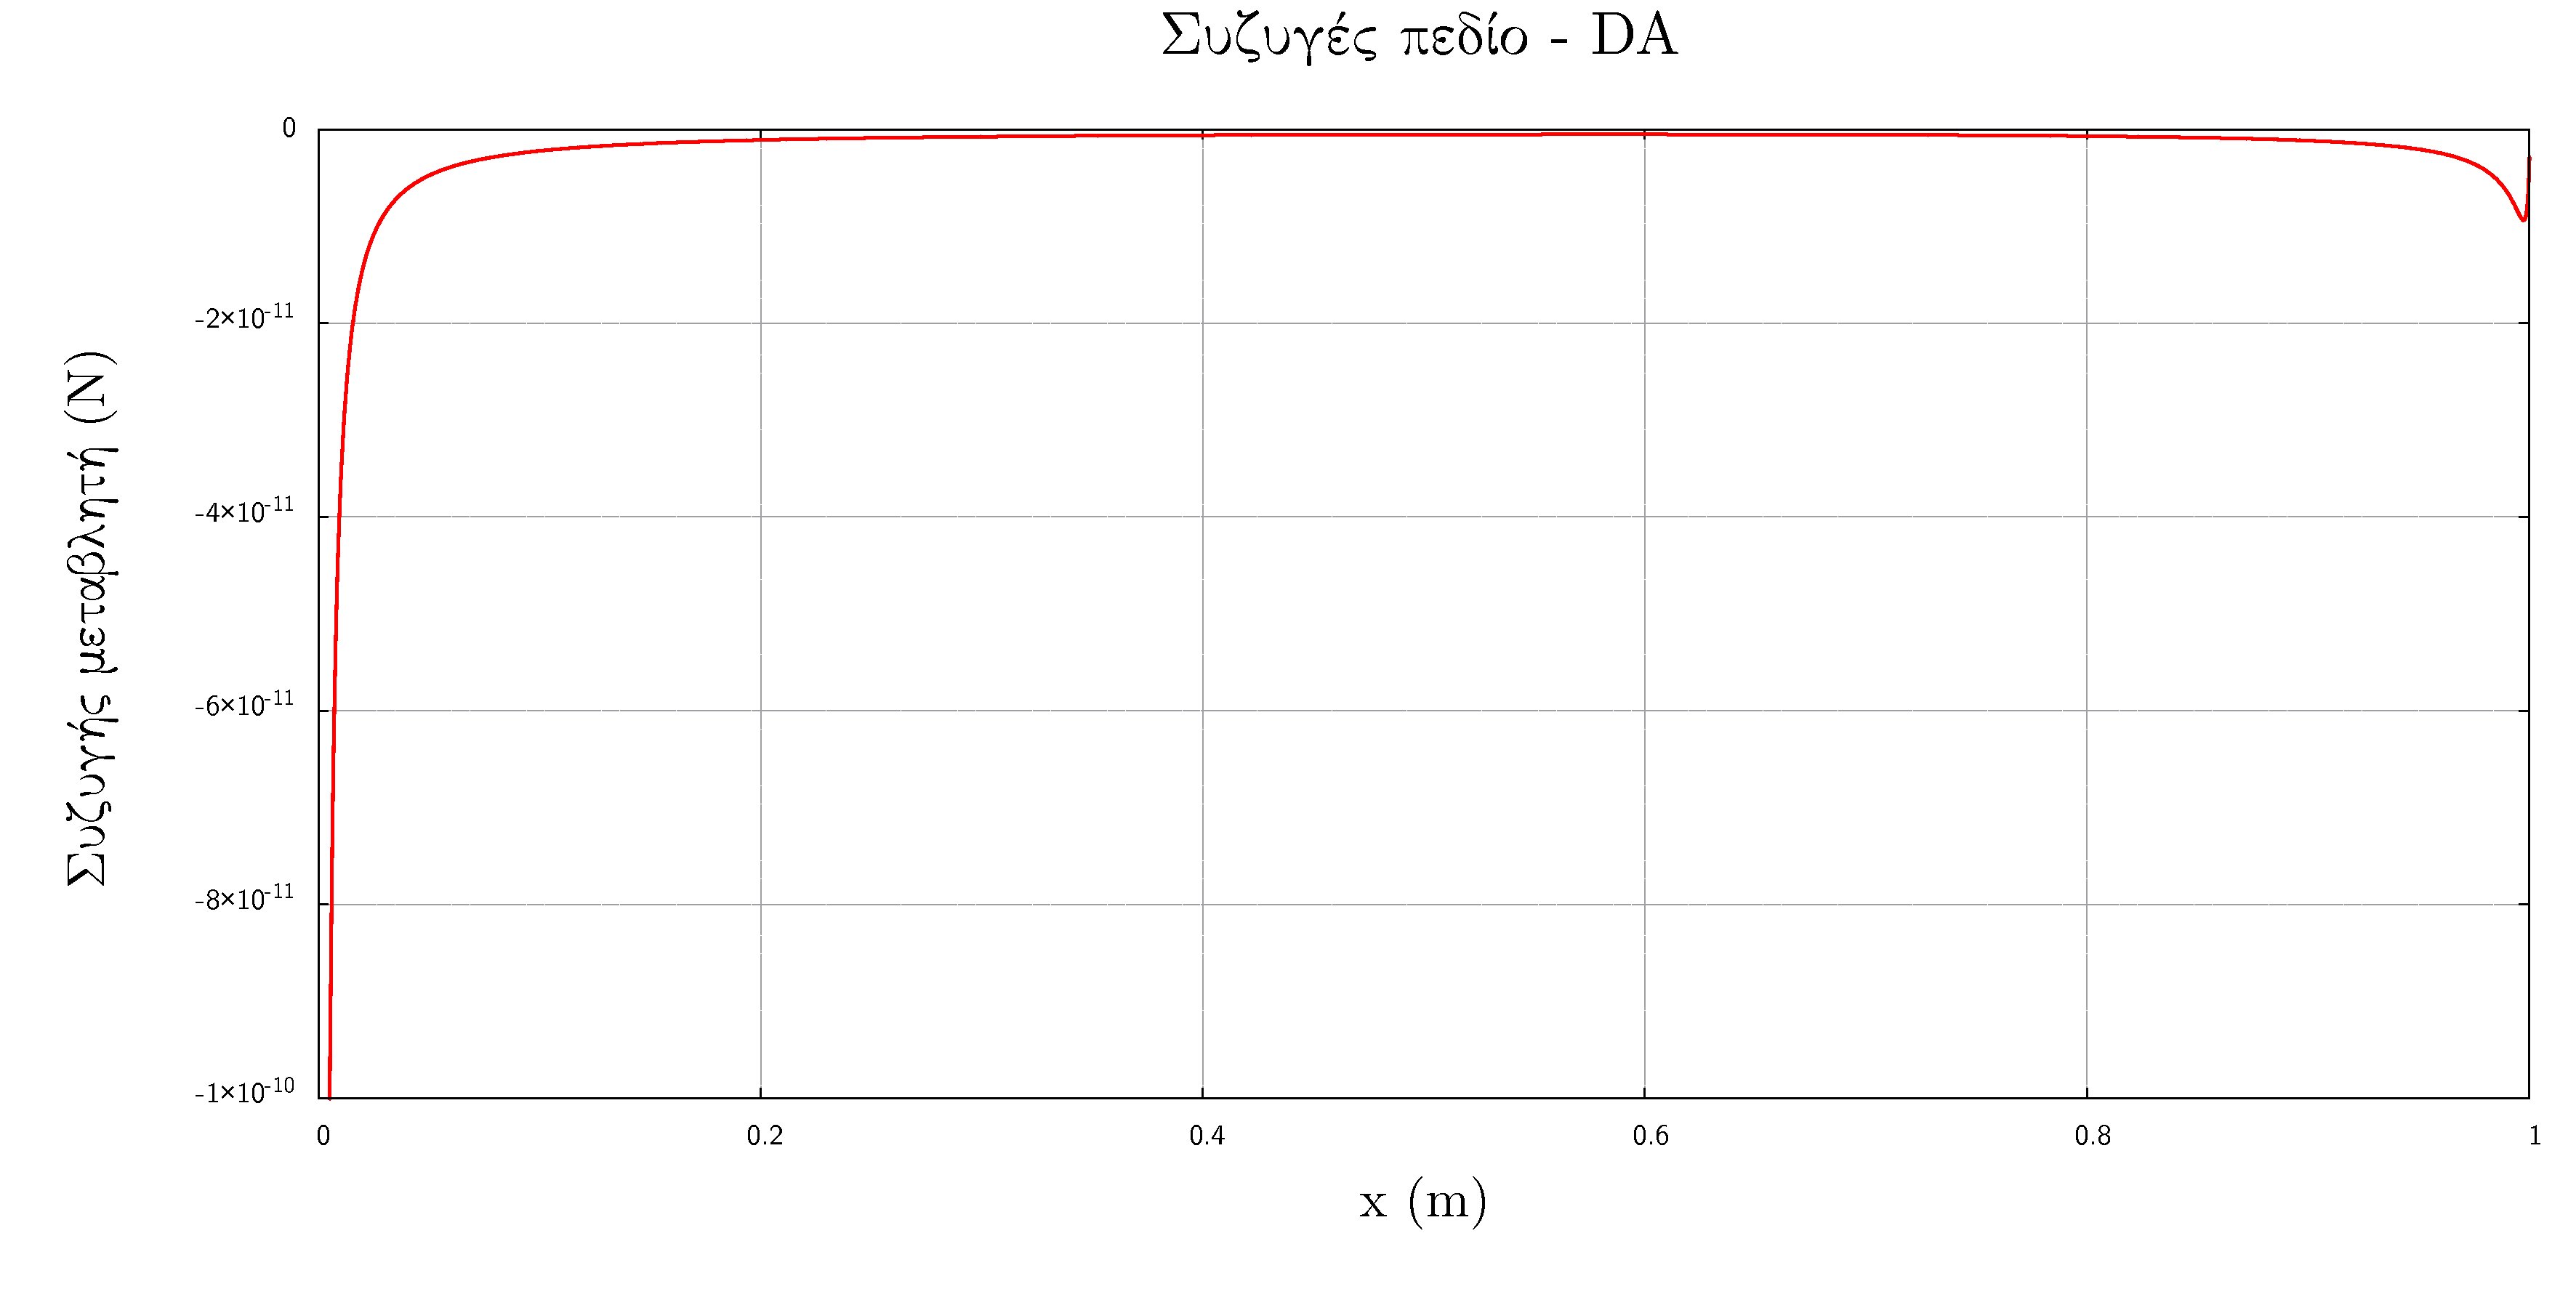
\includegraphics[width=0.9\textwidth]{figures/DA_field.pdf}
    \end{center}
    \caption{Συζυγές πεδίο με διακριτή συζυγή μέθοδο}
    \label{fig:DAfield}
\end{figure}

